% !TeX root = ../main.tex
\subsection{选题依据及研究意义}

世界模型（World Model）是智能体通过环境观测与交互经验建立的、用于表征外部世界状态及预测其演化规律的内部模型\cite{worldmodels2018,ref02}。现实环境持续变化，而智能体通常只能获得离散且不完整的观测信息，因此需要结合历史观测与交互经验，形成并维护对当前环境的内部估计，而不能只依赖单次观测。如图~\ref{fig:world-model-loop} 所示，世界模型通过感知信息持续更新内部状态，并在给定动作等条件下推演未来可能的环境变化；智能体则利用预测结果进行规划与行动，再通过实际执行反馈修正内部状态，形成感知、预测与行动相互联系的闭环。世界模型的内部状态可以采用潜在变量、视觉特征或显式三维结构等不同形式。不同表征形式在空间结构的显式程度、状态维护方式及预测信息保留方面各有侧重。因此，表征需要兼顾对当前环境的组织能力与对未来变化的支持能力。\textbf{作为空间智能与具身智能的重要基础，世界模型通过统一表征环境状态及其演化，连接环境理解、动作后果预测与自主规划。}

\begin{figure}[H]
  \centering
  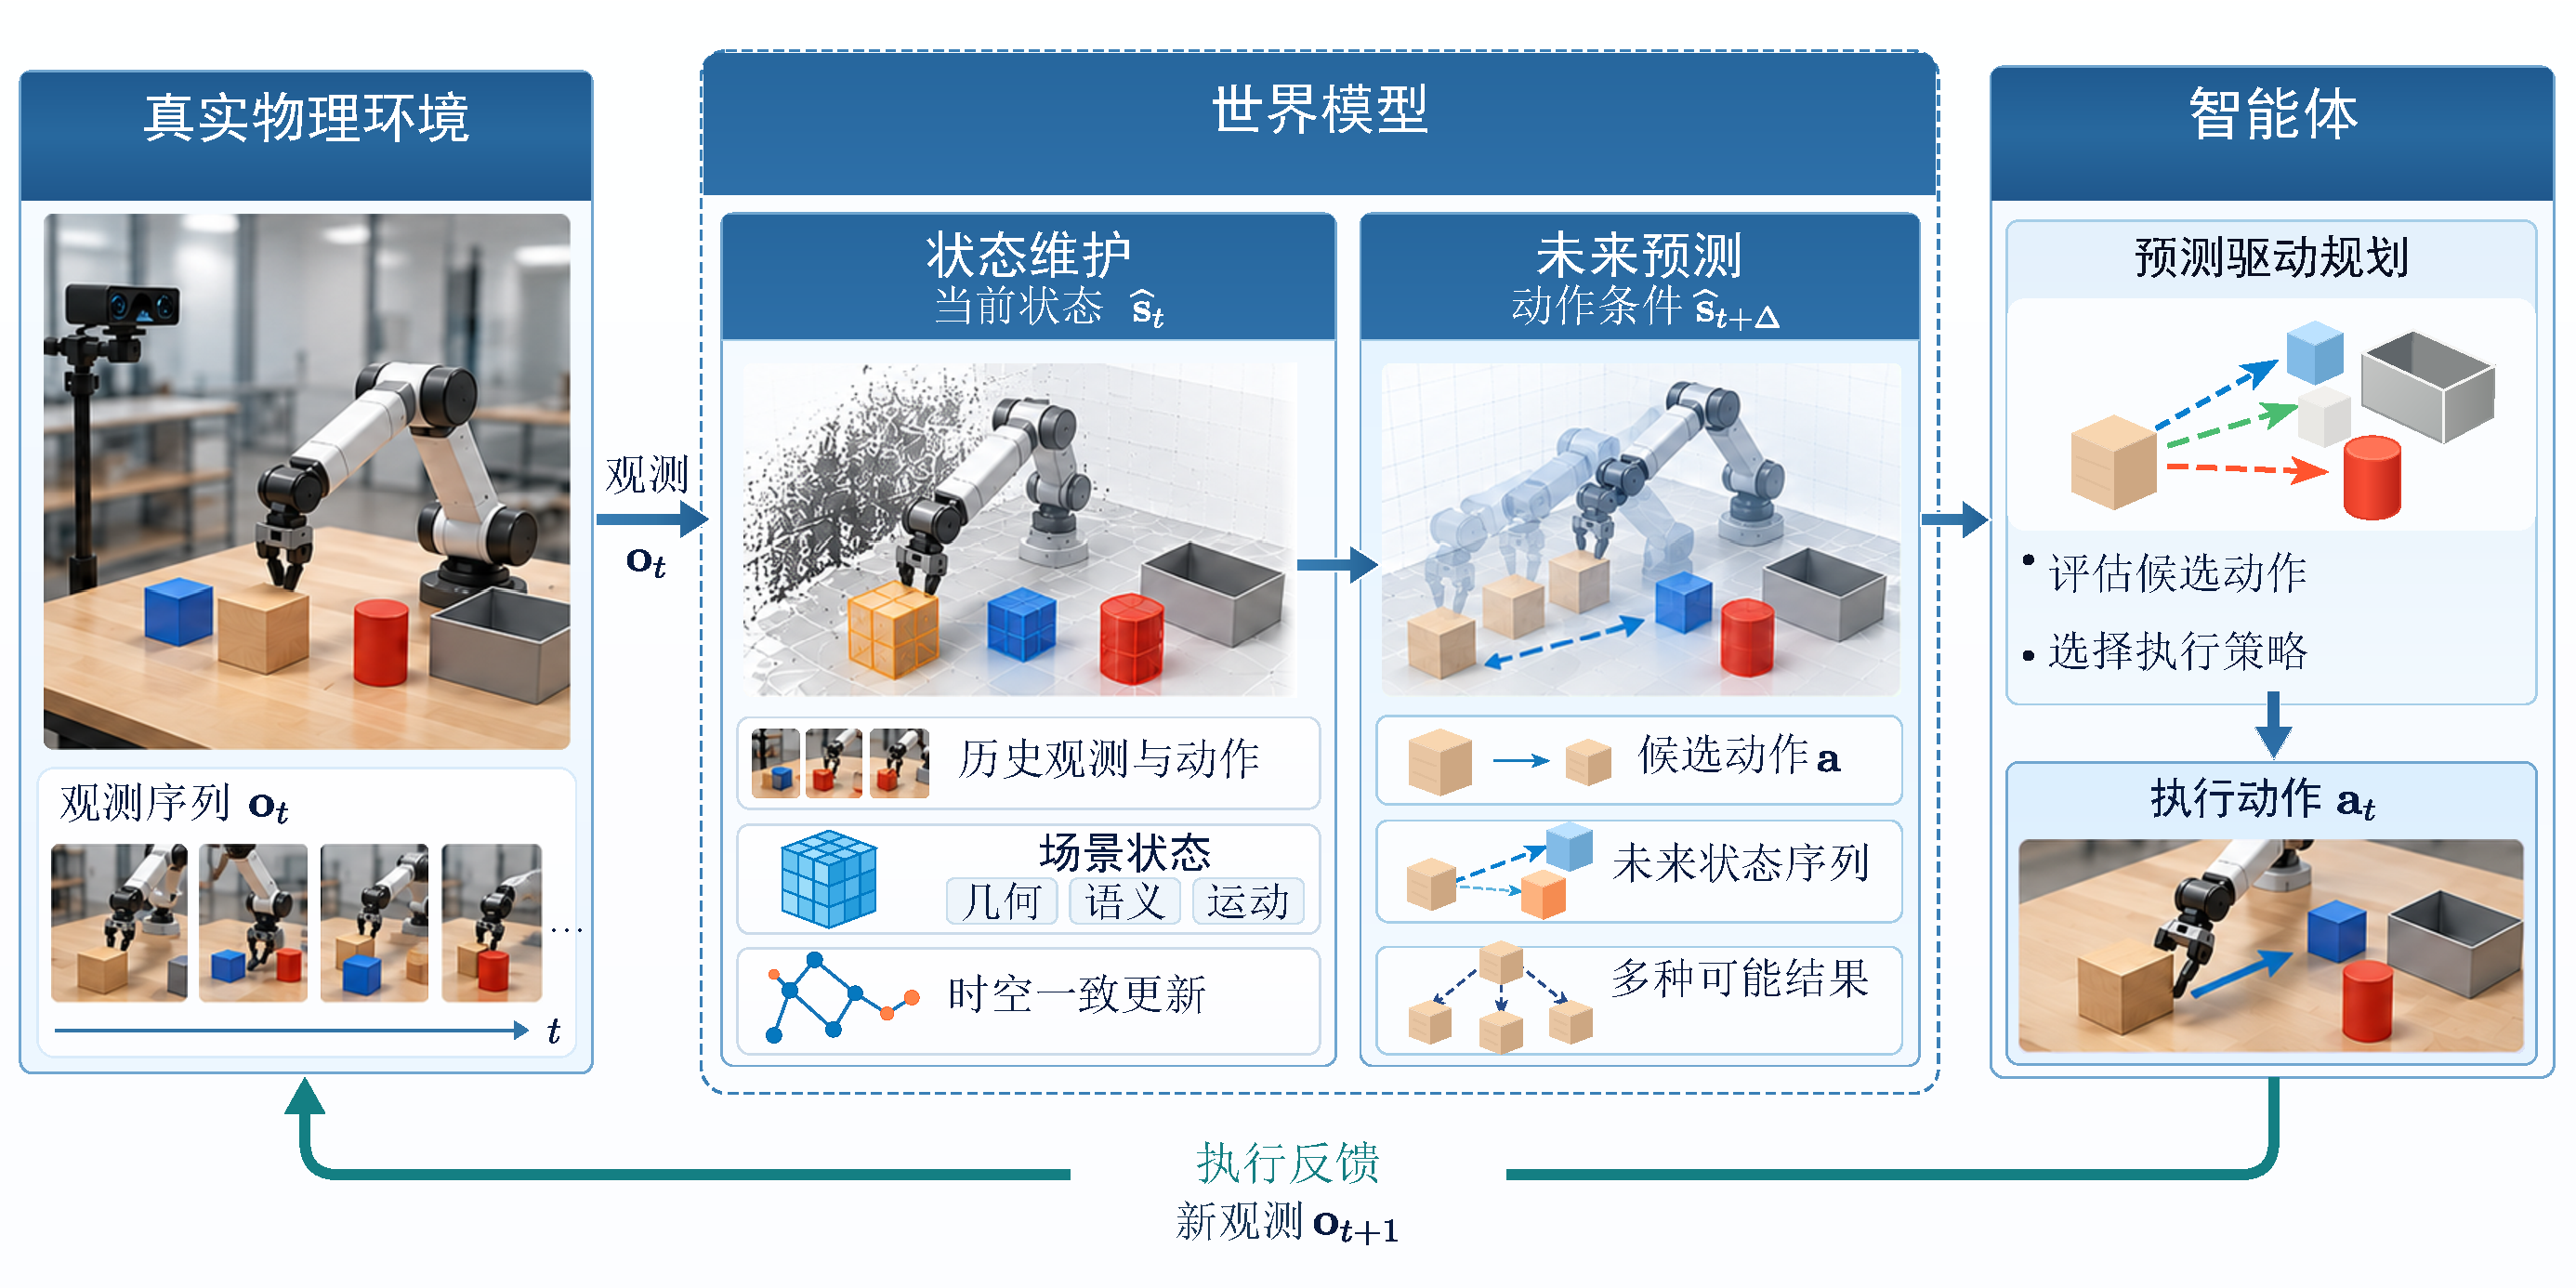
\includegraphics[width=0.98\linewidth]{figures/chapters/ch01-basis/world-model-loop/figure.pdf}
  \caption{世界模型与智能体的感知—预测—行动闭环示意}
  \label{fig:world-model-loop}
\end{figure}

世界模型已成为国际人工智能领域的重要前沿研究方向，也是推动人工智能从信息感知与内容生成走向物理世界理解、动态预测和自主决策的重要技术。国家自然科学基金委员会于2026年发布“空间智能与世界模型”专项项目申请指南，推动相关基础理论与关键技术研究\cite{nsfcworldmodel2026}；美国国家科学基金会（NSF）通过CAREER项目支持世界模型与机器推理等方向的研究\cite{nsfworldmodel2025}。工业界也在积极探索世界模型的技术潜力，Google DeepMind 推出 Genie 3，能够生成可实时交互的动态虚拟环境，探索世界模拟与智能体交互的结合\cite{deepmindgenie2025}；NVIDIA 发布 Cosmos 世界基础模型平台，面向机器人和自动驾驶等物理智能应用，支持环境生成与仿真研究\cite{nvidiacosmos2025}。这些科研布局与技术进展体现了世界模型在新一代人工智能基础研究和实际应用中的重要地位。

面向航天器在轨维护、无人系统自主作业等复杂任务，智能体需要在有限观测条件下持续理解动态环境，并预测自身行为可能引起的变化。美国国家航空航天局（NASA）开展的机器人在轨加注任务（Robotic Refueling Mission，RRM）为此类应用提供了实际案例：该项目利用国际空间站上的 Dextre 机器人，在地面远程操控下完成了保护覆层切割与翻起、线缆剪切、盖帽拆卸及阀门操作等技术演示，验证了复杂在轨机器人服务操作的可行性\cite{nasarrrm2026}。在轨维护之外，另一类需求来自自主空中操作。例如，搭载夹爪的无人机可自主接近并抓取目标，已有研究探索视觉语言引导的无人机抓取\cite{uavgrasp2026}。飞行运动带来的视角变化，以及近距离操作中的遮挡和目标状态变化，都要求智能体利用有限观测持续估计动态场景，并预测给定动作后的响应。不同场景对连续运动、对象关联、结构变化和动作预测的侧重并不相同；以下图示以在轨维护为例说明其中一类建模需求。

\begin{figure}[H]
  \centering
  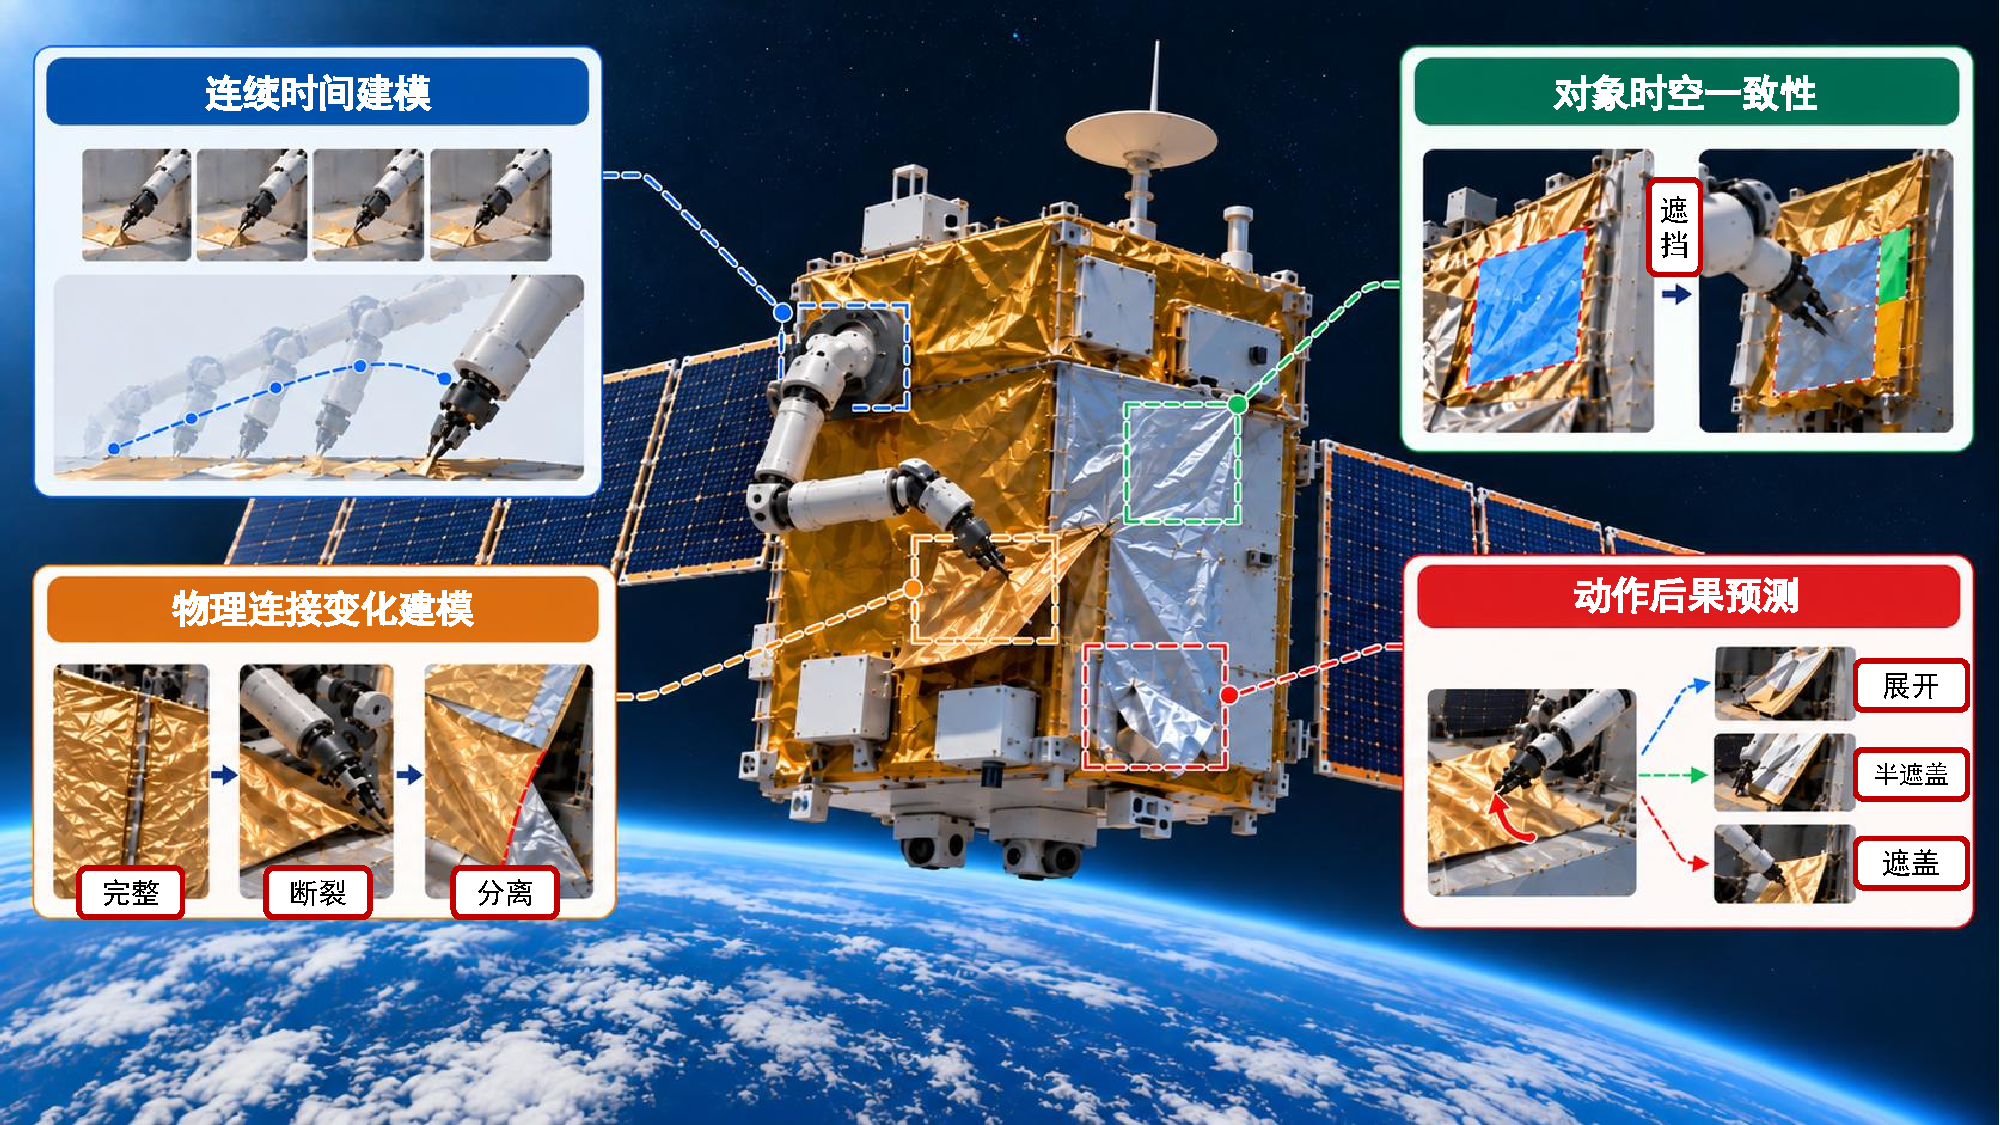
\includegraphics[width=0.98\linewidth]{figures/chapters/ch01-basis/spacecraft-maintenance/figure.pdf}
  \caption{复杂动态环境中的世界模型建模需求示例（以在轨维护为例）}
  \label{fig:spacecraft-manipulation}
\end{figure}

世界模型已在潜在状态预测、三维动态场景表征及动作条件演化预测等方面取得重要进展。面向观测不完备且持续变化的物理环境，现有不足可归纳为以下四个相互关联的问题：（1）运动连续而视觉观测离散，因此需要从稀疏观测中建立观测间可连续查询的运动表征，但非采样时刻的真实运动仍难由现有观测充分约束\cite{retimegs2026}；（2）遮挡、共动与形变要求持续维护对象身份及跨时刻关联，但仍易引发对象归属歧义\cite{consistentinstance2026}；（3）连接、装配或材料连续性改变后，需要重配置失效的跨部件约束并保留仍有效的历史，现有表征仍难兼顾二者\cite{gaustar2025}；（4）动作后果预测需要利用已有运动与当前有效结构关系，如何提高复杂动态条件下的预测准确性并厘清误差影响仍待研究\cite{ref06,phystwin2025}。这些问题分别为后文的连续运动恢复、对象时空一致性、结构约束关系变化下的表征维护和动作条件预测研究提供问题依据。

\textbf{在导师承担的国家自然科学基金青A项目和联合基金重点项目支持下，本课题面向复杂动态环境中有限视觉观测下的动态场景表征构建与演化预测需求，开展连续动态世界模型构建方法研究}。课题拟研究动态场景中连续运动、空间组织及结构约束关系的协同表征，建立能够随新观测持续修正的连续动态世界表征，并进一步探索基于该表征的动作后果预测方法，形成贯通环境感知、动态表征与未来演化预测的模型构建框架。研究有望为复杂动态环境中的时空一致性建模和动作响应预测提供方法基础，并为地面与空中自主智能体、空天无人系统及航空航天装备智能维护等应用提供技术支撑。

\subsection{国内外研究现状及发展态势}

\subsubsection{四维动态场景重建}

\begin{figure}[H]
  \centering
  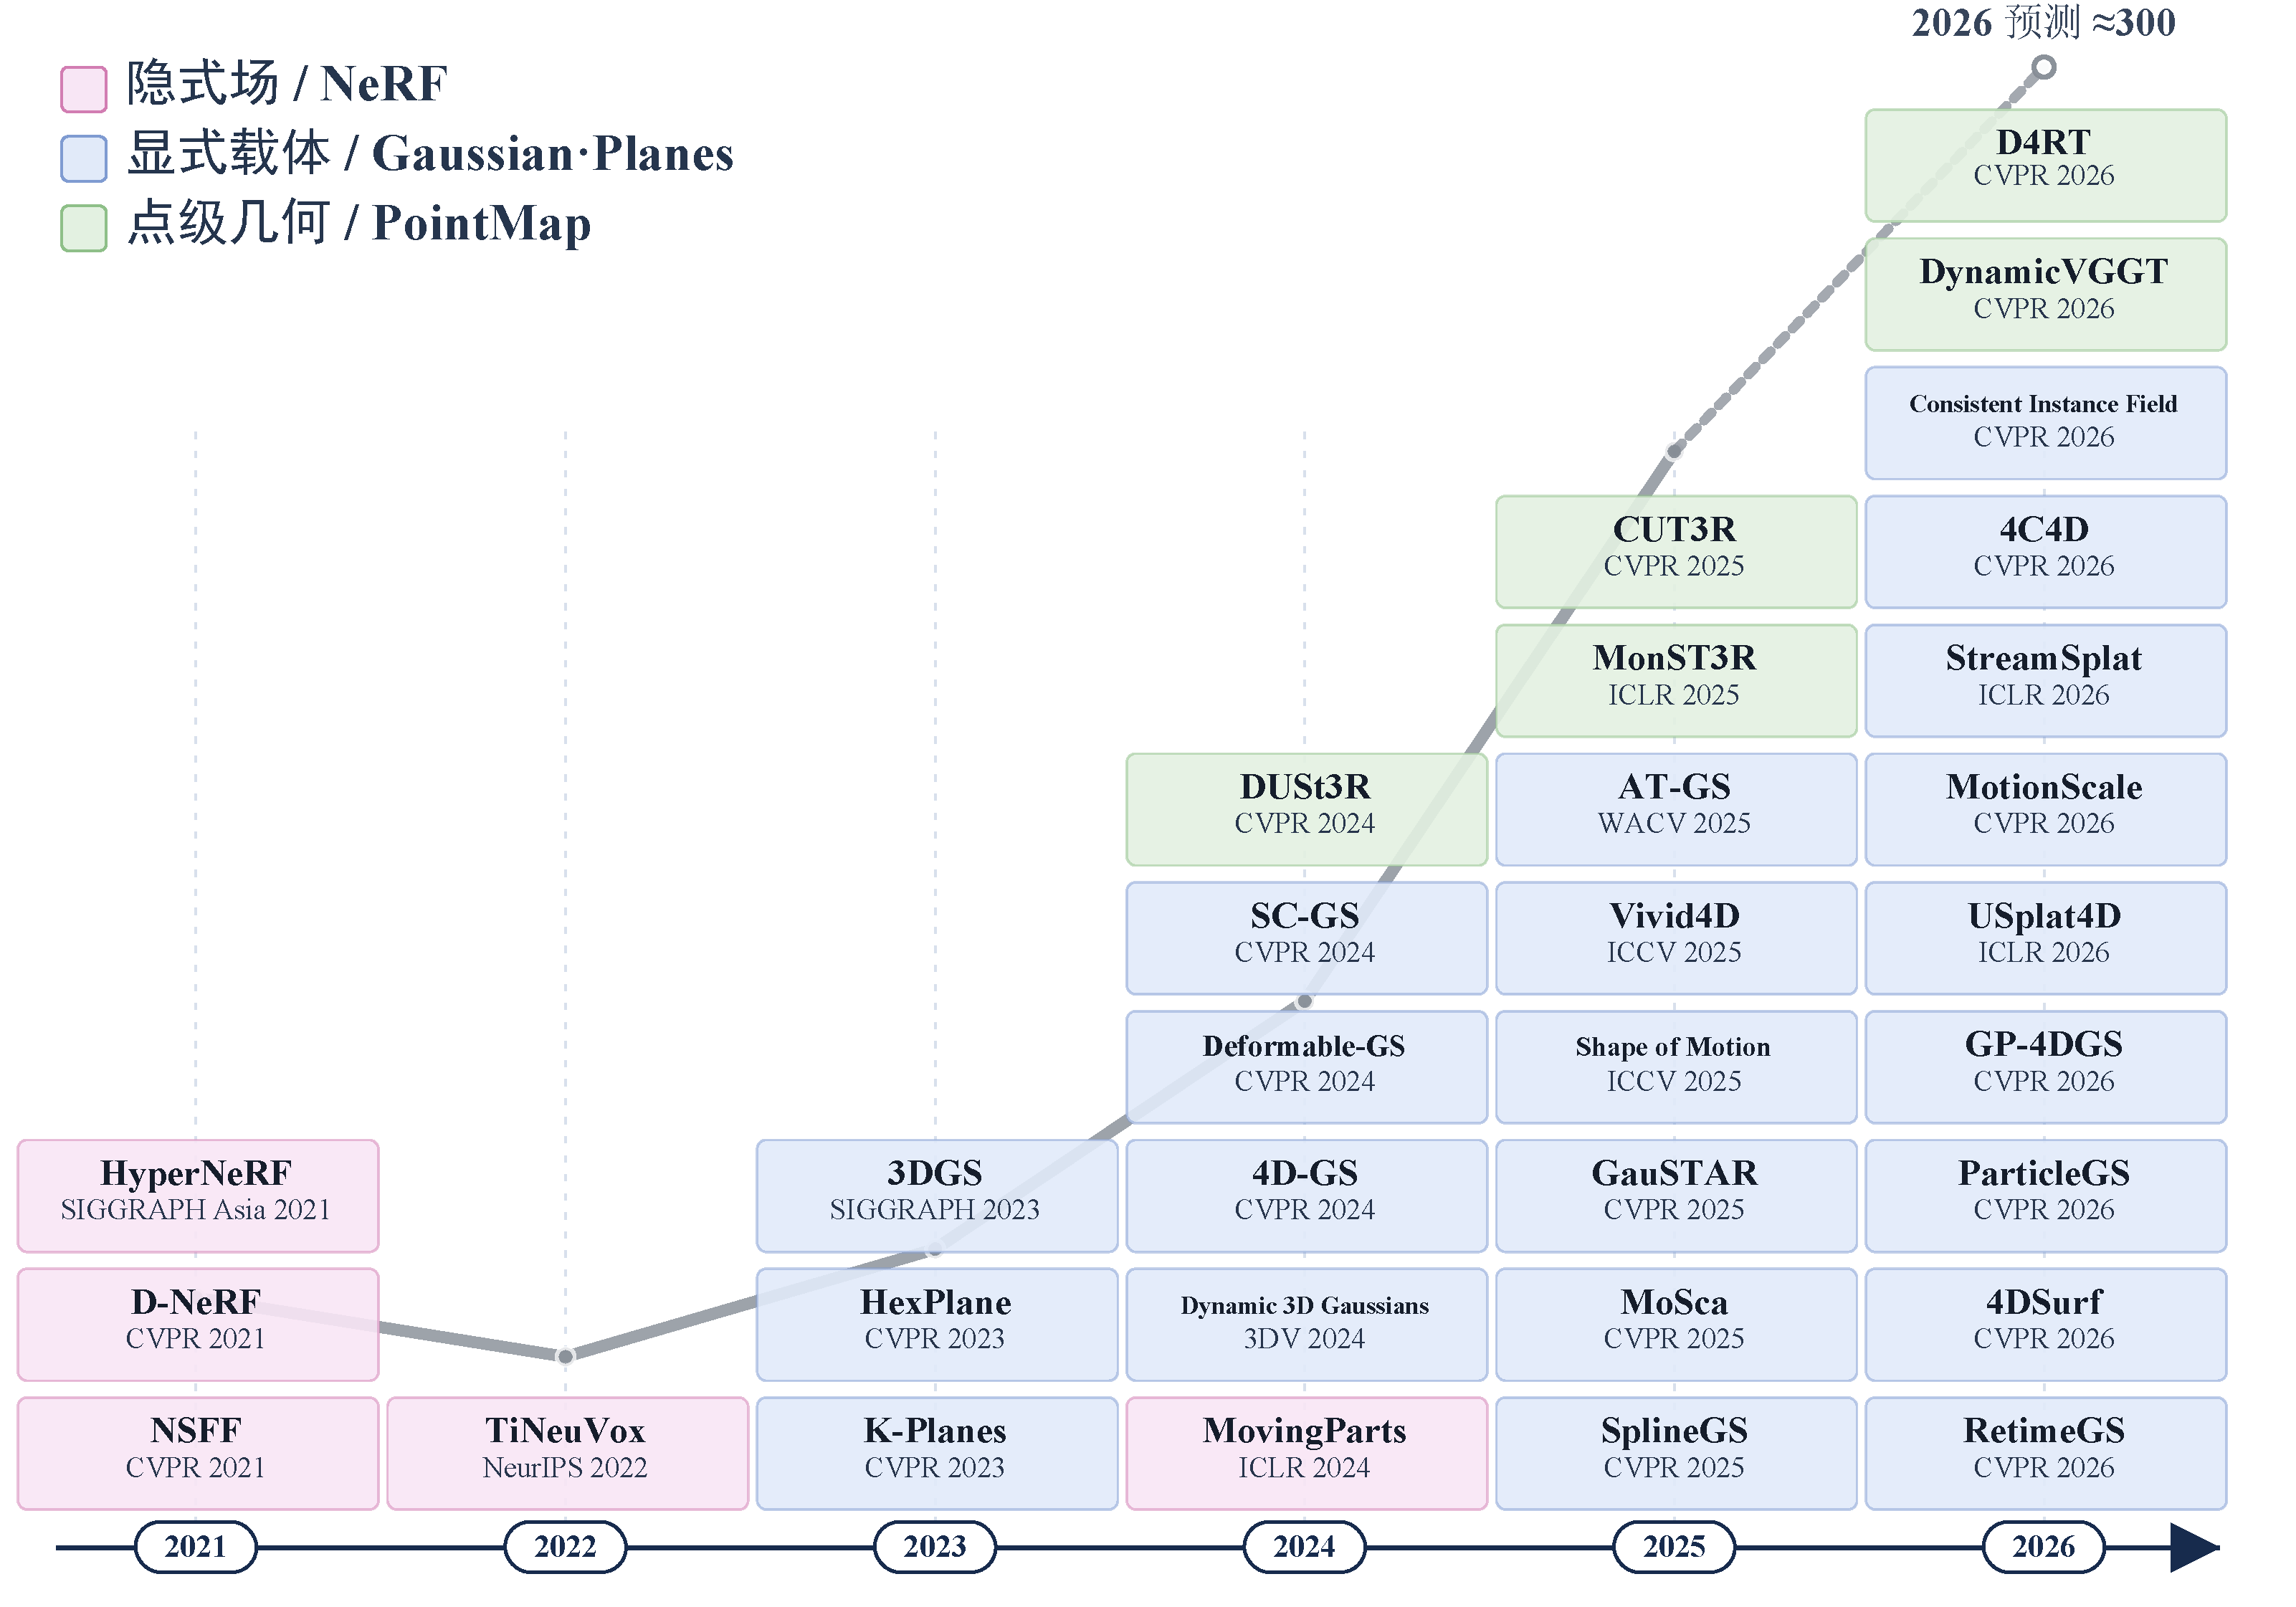
\includegraphics[width=\linewidth]{figures/chapters/ch01-basis/reconstruction-timeline/figure.pdf}
  \caption{四维动态场景重建的代表性工作与发展脉络}
  \label{fig:literature-evolution-reconstruction}
\end{figure}

四维动态场景重建从图像或视频恢复三维几何、外观及其时间变化，为运动分析和动态场景表征构建提供基础。相关研究已由动态几何恢复拓展至连续运动、跨时刻关联与结构更新\cite{cndynamic2024,cnnerf2025,cndynamicgs2026}。图~\ref{fig:literature-evolution-reconstruction} 按隐式场、显式图元和点级几何汇总了 2021—2026 年的代表性工作。

\textbf{隐式场表征}以连续函数描述几何与外观，并通过规范空间映射或形变建立时序联系。DynamicFusion 实现了非刚性动态表面融合与跟踪\cite{dynamicfusion2015}；D-NeRF、Nerfies、NSFF 和 HyperNeRF 则利用神经辐射场表达动态形变及拓扑变化\cite{nerf2020,dnerf2021,nerfies2021,nsff2021,hypernerf2021}。其运动恢复仍受观测覆盖、时序对应和形变假设约束，连续表达本身不能确定未观测时刻的真实运动。

\textbf{显式图元表征}以点、面元或高斯组织场景。3DGS 奠定了高效显式表示与可微渲染基础\cite{gs2023}；Dynamic 3D Gaussians、4D-GS、Deformable 3D Gaussians 和 SC-GS 探索持久跟踪、时变形变及稀疏运动控制\cite{dynamicgs2024,gs4d2024,deformablegs2024,scgs2024}，RetimeGS、SplineGS 和 ParticleGS 进一步研究连续时间重建、样条运动及物理外推\cite{retimegs2026,splinegs2025,particlegs2026}。

显式重建也开始处理空间组织、结构变化与观测不确定性：MoSca、Shape of Motion 和 MovingParts 利用运动组织跨时刻几何及部件关系\cite{ref05,shapeofmotion2025,movingparts2024}；Consistent Instance Field 维护对象身份与可见性\cite{consistentinstance2026}；GauSTAR 和 USplat4D 分别研究拓扑变化下的局部重建及不确定性引导的运动传播\cite{gaustar2025,usplat4d2026}。几何拓扑、对象身份、装配约束和材料连续性并非同一信息，仍需结合观测加以区分。

\textbf{点级几何表征}借助视觉基础模型直接预测三维几何与跨时刻对应。DUSt3R 和 VGGT 联合预测点图、深度及相机参数\cite{dust3r2024,vggt2025}；MonST3R、CUT3R 和 D4RT 将学习式几何扩展至动态视频、连续感知及时空查询\cite{monst3r2025,cut3r2025,d4rt2026}。这类方法提供了几何与运动先验，但预测结果如何形成可持续修正的时空一致表征，仍待研究。

总体而言，隐式场、显式图元和点级几何分别侧重连续表达、局部操作及学习式几何恢复；DyCheck、TAP-Vid、TAPVid-3D 和 PointOdyssey 提供了动态重建与点跟踪评价依据\cite{dycheck2022,tapvid2022,tapvid3d2024,pointodyssey2023}；Syn4D 进一步提供多视角合成视频及稠密几何、跟踪真值\cite{syn4d2026}。有限观测下如何协调运动、对象组织与结构变化，并持续维护有效历史，仍是关键问题。


\subsubsection{世界模型}

世界模型从环境观测与交互中构建内部状态并学习其演化，以支持预测和决策。研究路线已由潜在动力学、视觉表征预测拓展至生成式模拟和结构化三维建模。图~\ref{fig:literature-evolution-worldmodel} 汇总了 2018—2026 年的代表性工作及论文数量趋势（含 2026 年预测）；OpenAlex 检索结果用于观察领域发展\cite{savostyanov2026}。

\begin{figure}[htbp]
  \centering
  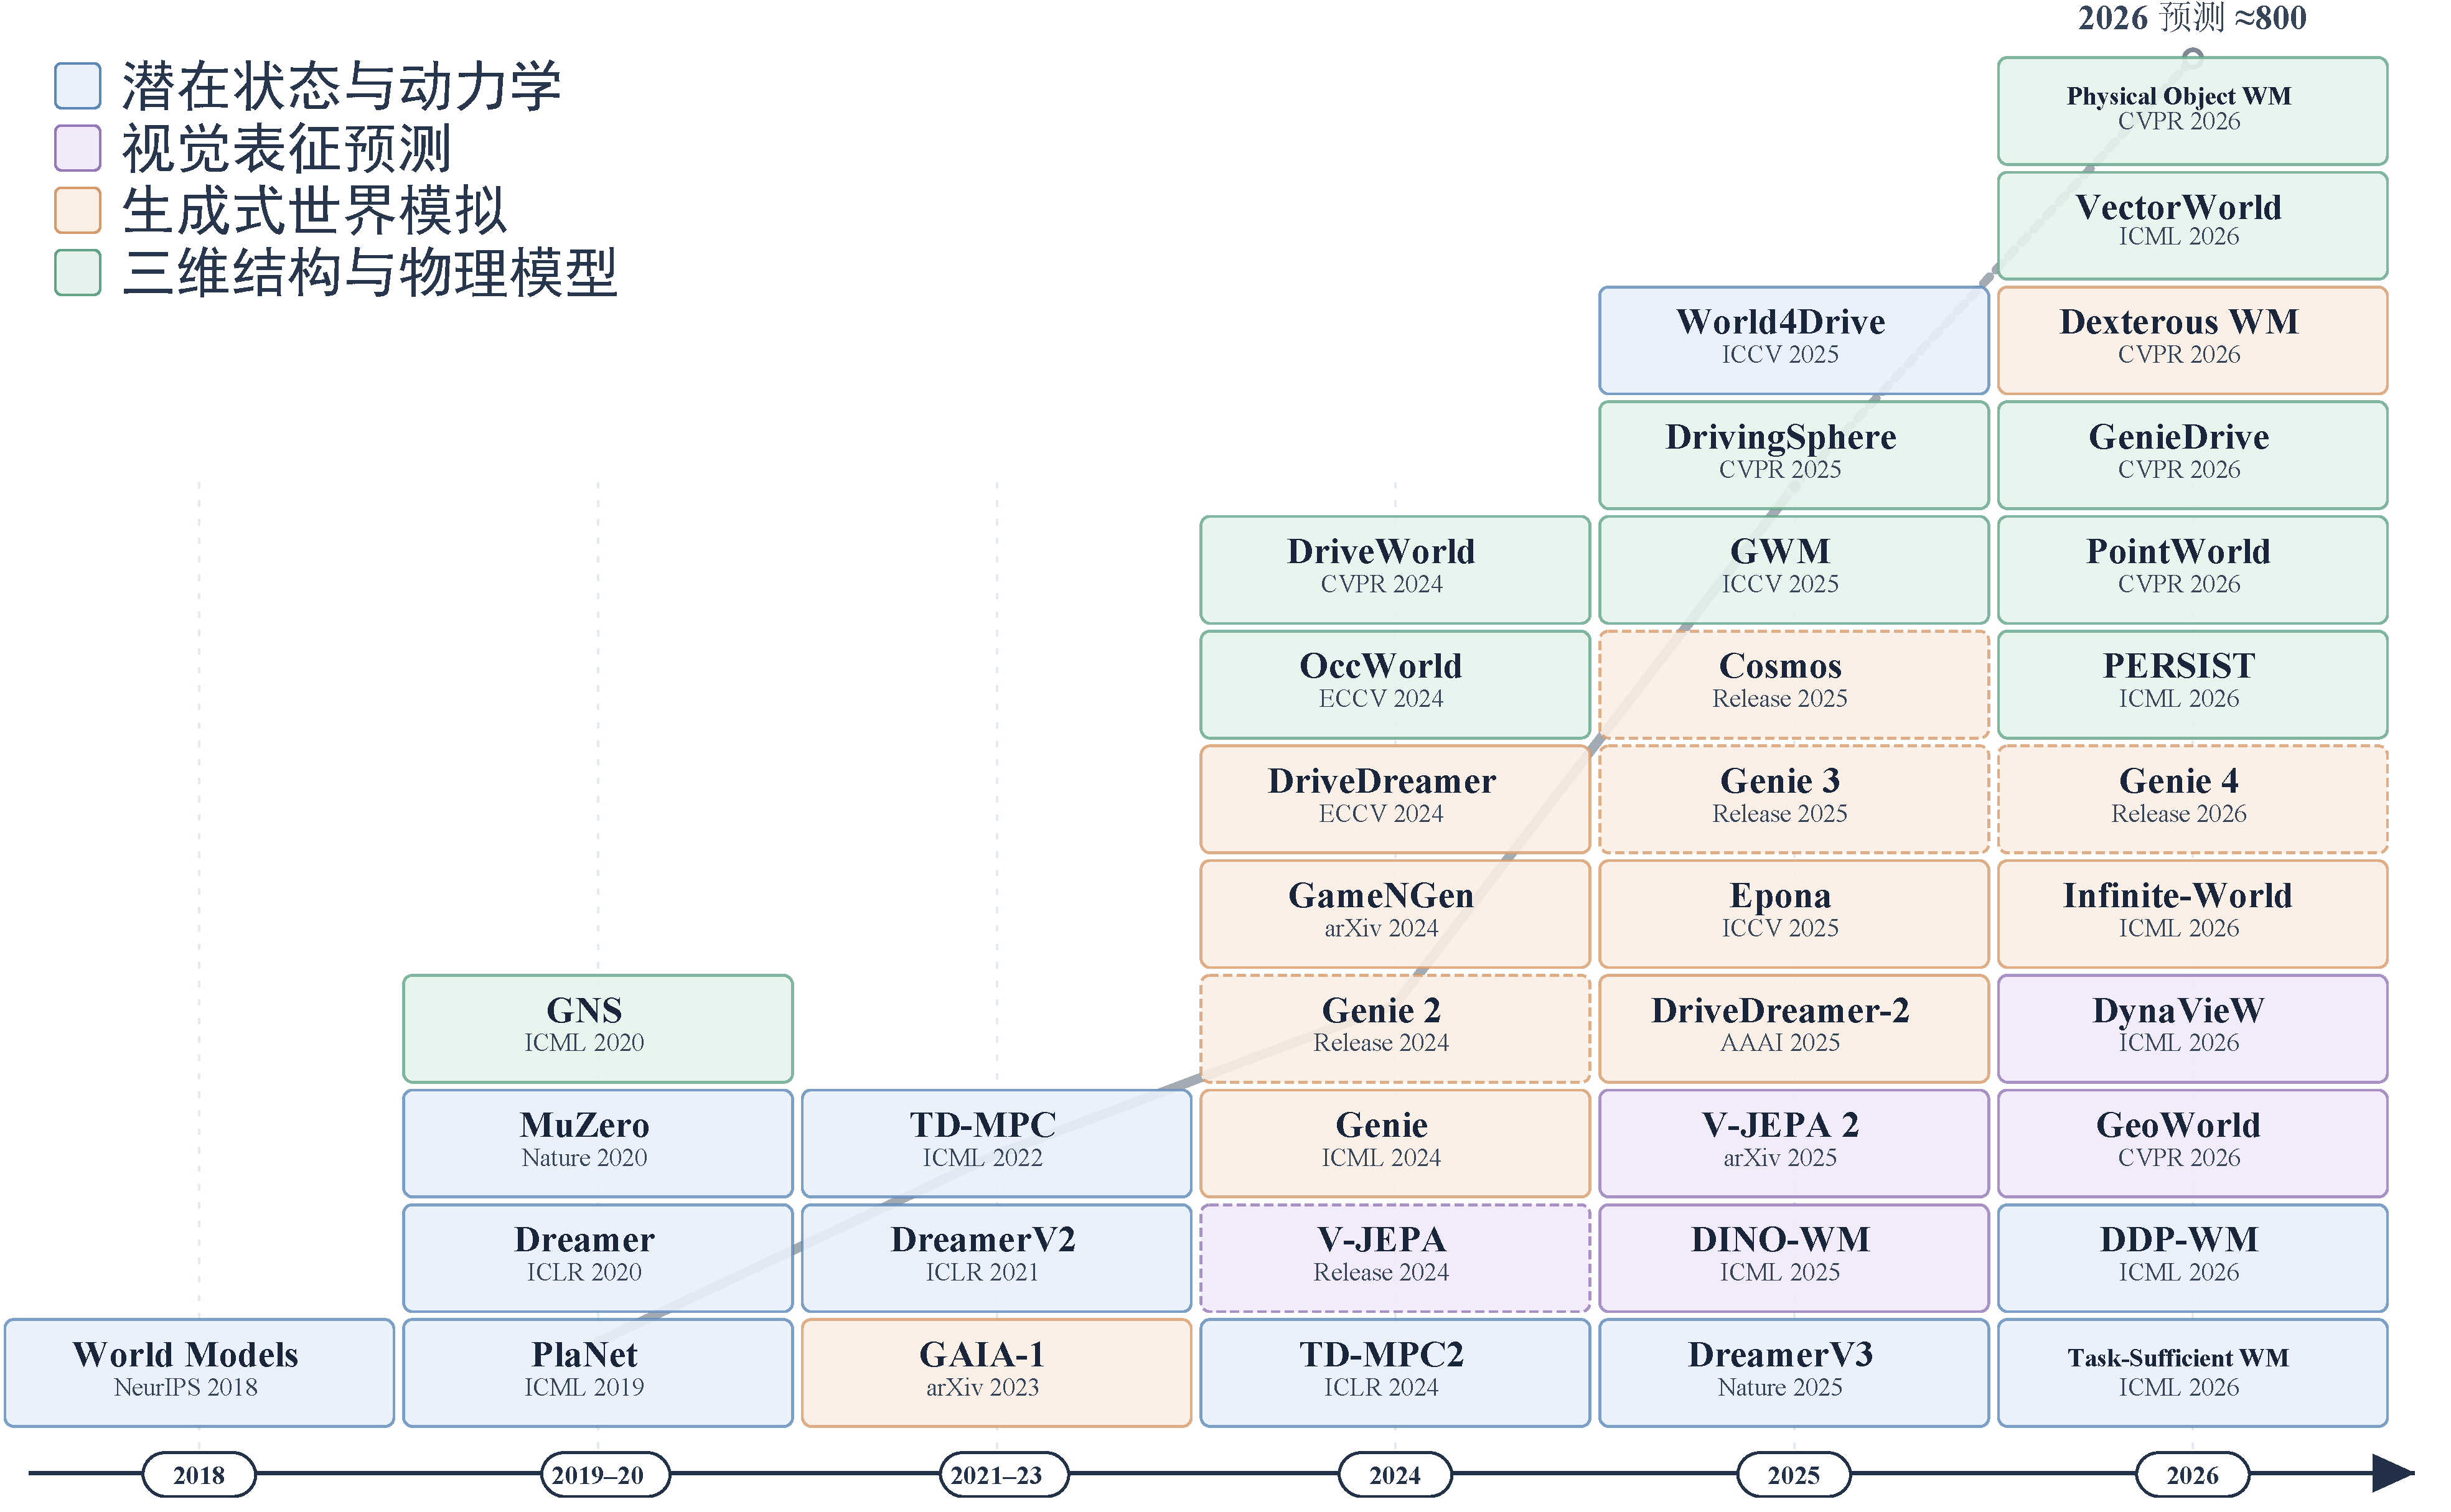
\includegraphics[width=\linewidth]{figures/chapters/ch01-basis/world-model-evolution/figure.pdf}
  \caption{世界模型的代表性工作与研究发展趋势}
  \label{fig:literature-evolution-worldmodel}
\end{figure}

\textbf{潜在状态与动力学模型}将历史观测和动作编码为紧凑状态并学习其转移。World Models、PlaNet、Dreamer 和 MuZero 探索循环记忆、潜在空间规划、想象学习及规划相关状态\cite{worldmodels2018,ref01,dreamer2020,muzero2020}；PETS、TD-MPC2、DreamerV3 和 Task-Sufficient World Models 延伸至不确定性建模、连续控制、多任务学习及任务充分表征\cite{pets2018,tdmpc2_2024,ref02,tasksufficientwm2026}。这类状态利于预测和规划，但不必然具备明确的三维几何、对象关联或物理结构含义。

\textbf{视觉表征预测模型}在视觉特征或对象级状态中预测未来：I-JEPA 学习语义表征，SAVi 与 SlotFormer 建模对象及其演化\cite{ijepa2023,savi2022,slotformer2023}；DINO-WM 和 V-JEPA 2 将预训练视觉特征用于动作条件预测与规划\cite{ref03,vjepa2_2025}；FR3D、Flow Equivariant World Models 及多视角掩蔽世界模型进一步探索三维潜在状态、运动记忆和多视角信息\cite{ref07,ref08,mvmwm2023}。其表征变化与真实几何、运动及物理关系的一致性仍需验证。

\textbf{生成式世界模拟模型}以未来图像、视频或交互环境为预测对象。Genie、GameNGen 和 Genie 2 探索从视频学习交互及生成环境\cite{genie2024,gamengen2024,deepmindgenie2_2024}；DriveDreamer、DriveDreamer-2 和 Epona 面向驾驶场景生成与预测\cite{drivedreamer2024,drivedreamer2_2025,epona2025}；Cosmos、Genie 3、Genie 4 和 Infinite-World 进一步推进物理场景、实时交互及长序列生成\cite{nvidiacosmos2025,deepmindgenie2025,deepmindgenie4_2026,infiniteworld2026}。生成质量仍不能替代对三维运动、物理约束和长期状态一致性的检验。

\textbf{三维结构与物理世界模型}以显式空间状态学习动态演化。GNS 建模粒子物理，OccWorld 和 GenieDrive 使用三维或四维占据预测驾驶场景\cite{gns2020,occworld2024,geniedrive2026}；PhysTwin、GWM 和 PointWorld 分别研究可变形物理对象、高斯动态表示及点流动作预测\cite{phystwin2025,gwm2025,ref06}；PERSIST 与 VectorWorld 探索持久三维状态和结构化流式建模\cite{ref10,vectorworld2026}。当前关键问题是如何结合连续运动历史与有效结构，持续维护动态场景表征并支持动作响应预测。

总体来看，世界模型从紧凑潜在状态和视觉预测延伸至生成式模拟及结构化三维建模，但不完整观测下的表征持续维护，以及运动、对象归属、结构约束关系和交互历史对动作预测的作用仍待明确。



\subsubsection{具身操作中的动作学习}

具身操作中的动作学习根据视觉观测、机器人状态及任务要求生成动作，连接环境感知与交互。相关研究已由直接动作预测扩展至预测辅助决策和世界—动作联合建模\cite{cnvla2026}。图~\ref{fig:literature-evolution-action} 汇总了 2020—2026 年的代表性工作。

\begin{figure}[H]
  \centering
  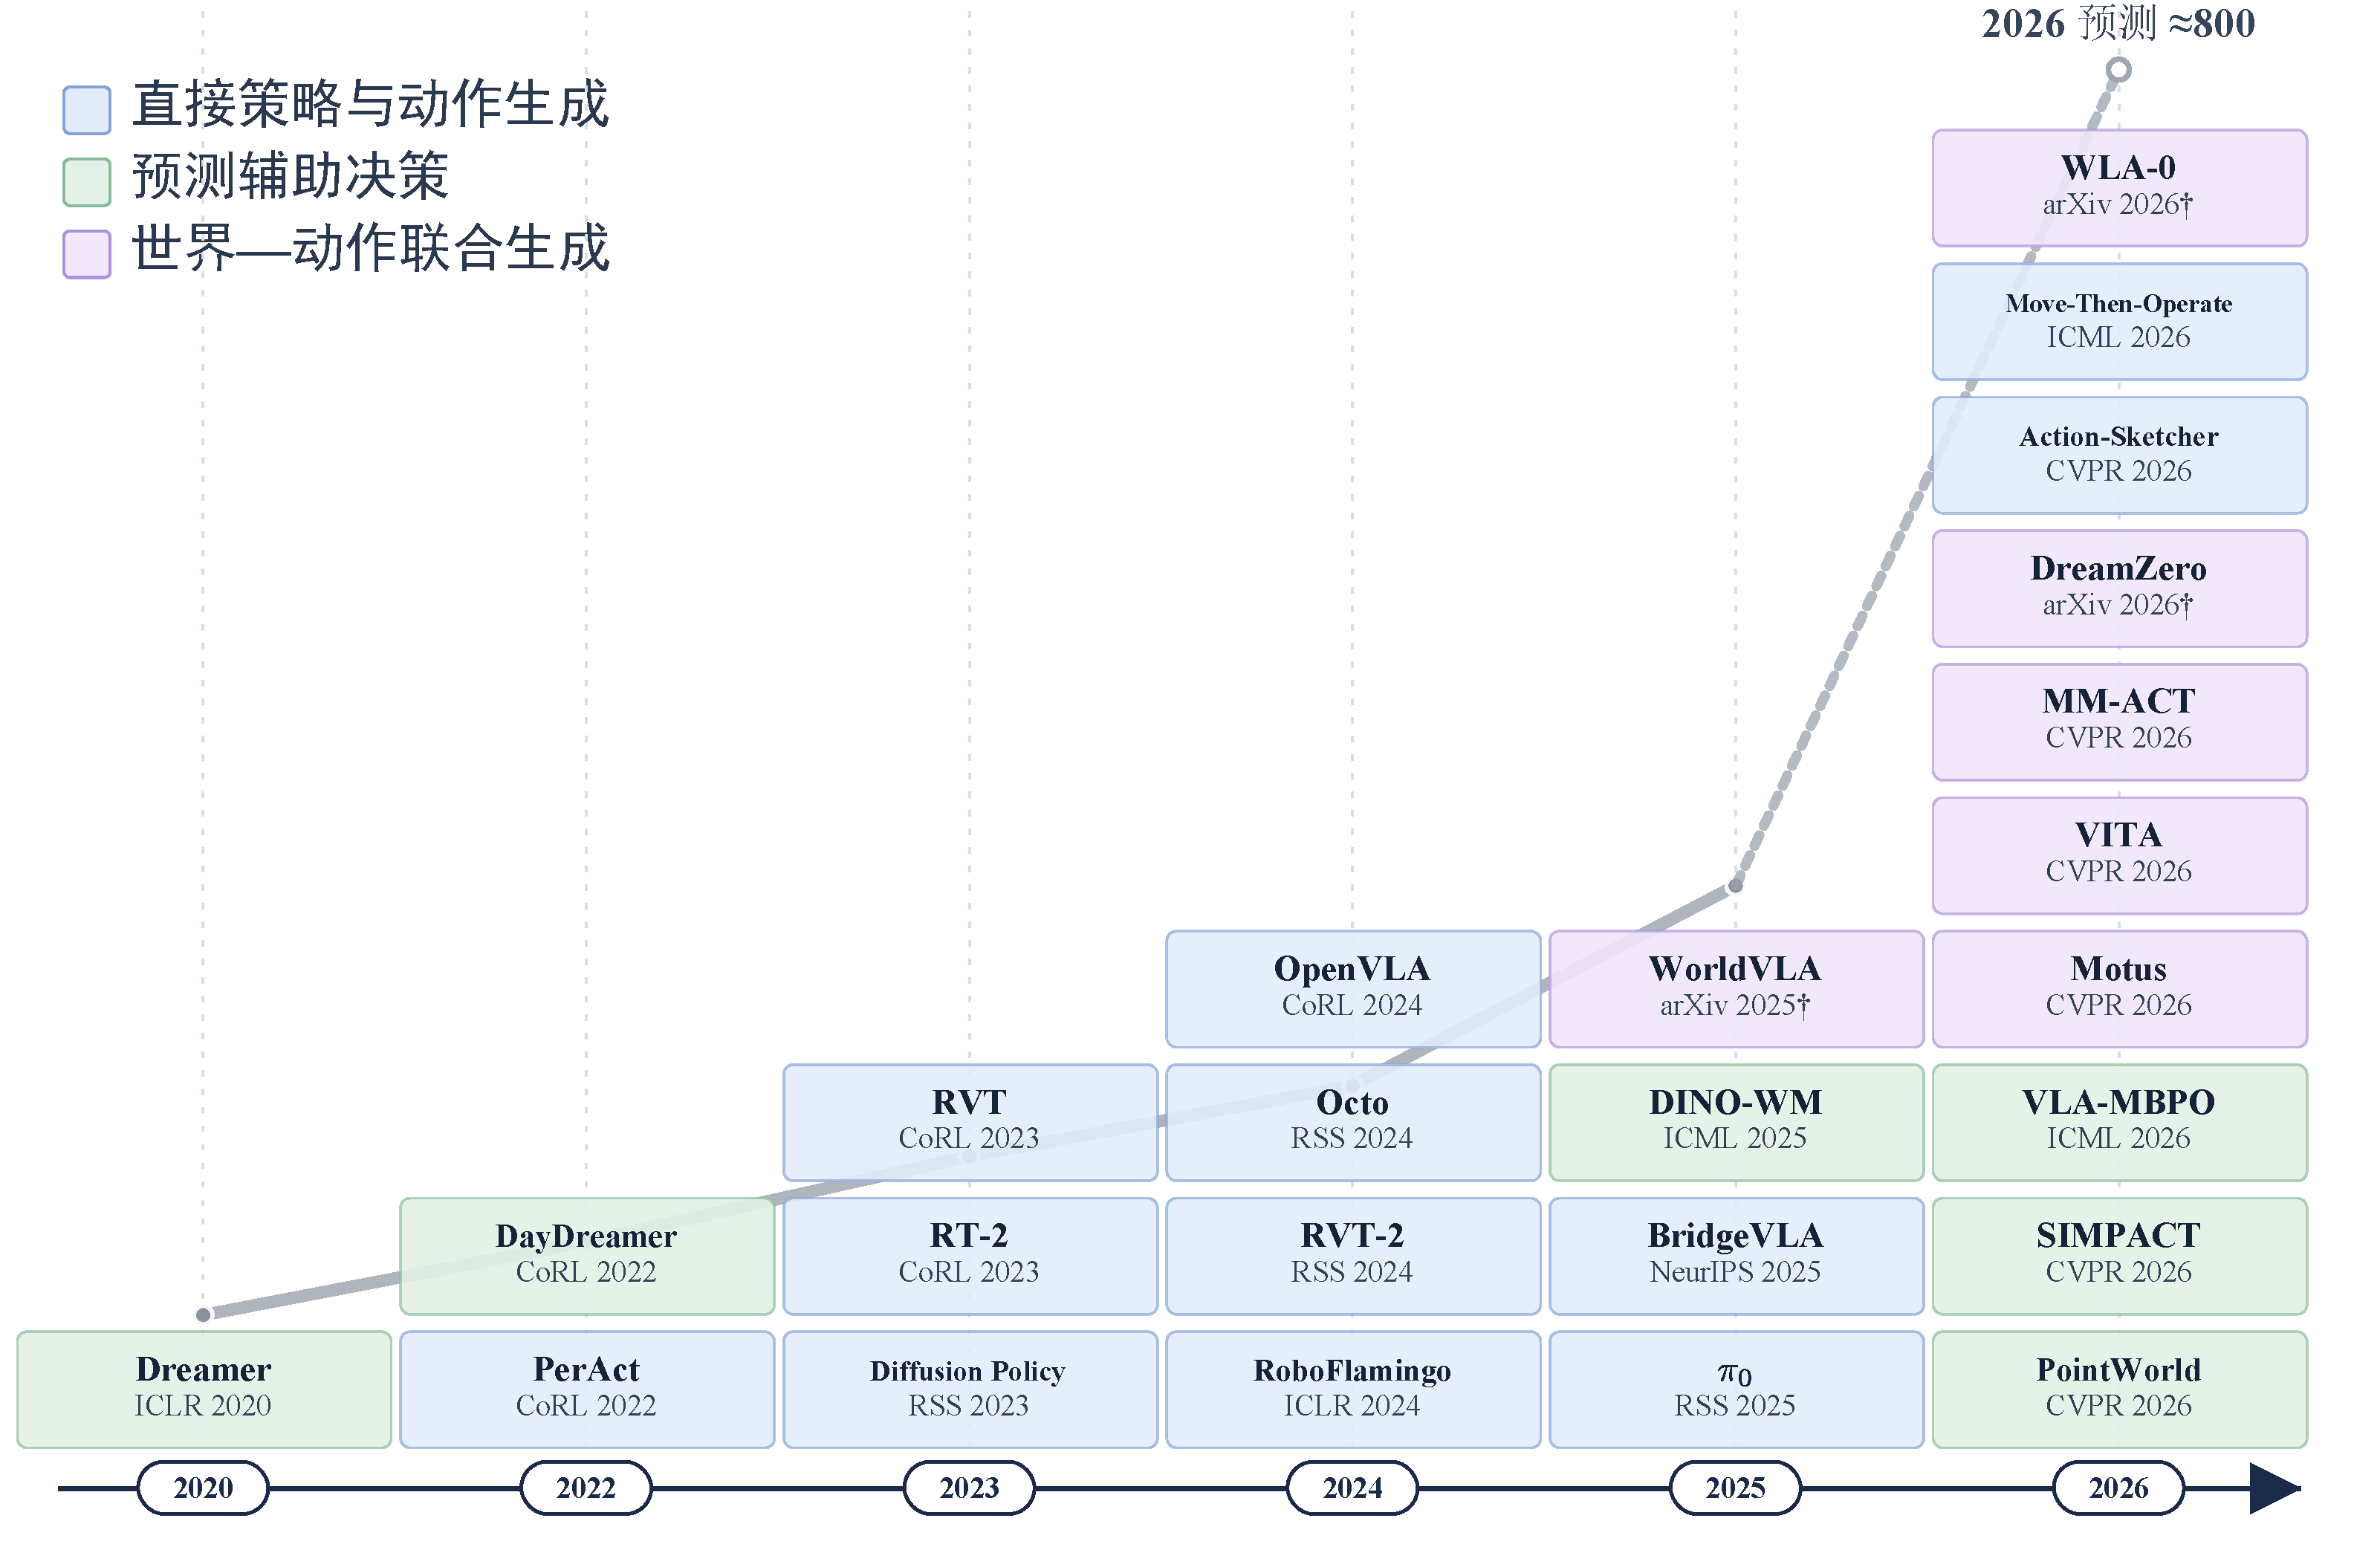
\includegraphics[width=\linewidth]{figures/chapters/ch01-basis/action-learning-timeline/figure.pdf}
  \caption{具身操作动作学习的代表性工作与发展脉络（† 表示预印本）}
  \label{fig:literature-evolution-action}
\end{figure}

\textbf{直接策略与动作生成}学习从视觉、语言及机器人状态到动作的映射。RT-2 和 OpenVLA 将视觉语言模型用于机器人动作生成\cite{rt22023,openvla2025}；Diffusion Policy 和 $\pi_0$ 探索连续动作建模，RoboFlamingo、PerAct、RVT-2 和 BridgeVLA 则结合时序、体素、多视角或三维表征增强空间感知与操作能力\cite{diffusionpolicy2025,pi02025,roboflamingo2024,peract2023,rvt22024,ref12}。此类策略不必显式恢复连续运动、对象关联和物理结构。

\textbf{预测辅助决策}利用未来状态支持动作选择与规划：Dreamer 在潜在空间学习想象轨迹\cite{dreamer2020}，DINO-WM 预测动作条件下的视觉变化\cite{ref03}，PointWorld 则以三维点流预测运动\cite{ref06}。预测表征能否保留影响动作响应的信息、并转化为任务收益，仍需在具体交互条件下检验。

\textbf{世界—动作联合生成}在统一模型中预测环境演化与动作。WorldVLA 自回归生成未来图像和机器人动作\cite{worldvla2025}，DreamZero 联合学习未来视频与动作\cite{dreamzero2026}；其生成与动作的一致性仍需通过执行反馈及物理状态评价验证。

DROID 和 REASSEMBLE 提供真实机器人操作或接触密集型拆装记录；IMPACT 提供工业装配的五视角同步采集及组件状态标注；PhysTwin 和 Deform360 则覆盖可变形对象交互与多视角触觉观测\cite{droid2024,reassemble2025,impact2026,phystwin2025,deform3602026}。RLBench、LIBERO、CALVIN、RoboCasa、RoboTwin 和 SIMPLER 支持多任务及仿真评价\cite{rlbench2020,libero2023,calvin2022,robocasa2024,robotwin2025,simpler2025}；数据间的观测、动作和任务协议存在差异。

总体而言，动作研究由直接策略拓展至预测辅助和世界—动作联合建模。连续运动、对象归属及当前有效结构约束能否改善动作后果预测，并在一致交互条件下带来收益，仍需验证。


\subsubsection{总结}

综上，四维动态场景重建已从几何与外观恢复拓展到连续运动、跨时刻对象关联和结构变化建模；世界模型由潜在动力学与视觉特征预测发展到生成式模拟及结构化三维建模；具身动作学习也由直接策略扩展至预测辅助决策和世界—动作联合生成。相关方法与数据基准为动态环境表征、演化预测和交互决策提供了基础。

然而，现有研究多围绕各自任务展开，重建或生成效果尚不能说明表征是否保留了动作响应所需的信息。有限离散观测下的连续运动与场景结构仍可能存在歧义，遮挡或共动条件下的对象归属，以及结构约束关系变化后的约束重配置和有效历史延续仍待研究；连续运动、对象归属及当前结构关系如何影响动作后果预测和误差传递，也缺乏可比分析。针对上述不足，本项目拟研究不完备观测下\textbf{连续运动与场景结构的可区分条件}，构建能够适应结构约束关系变化的动态场景表征，并分析其对\textbf{动作响应预测的支持作用及误差传递机理}。

\subsection{已有工作积累及研究基础}

\noindent\textbf{（1）基于稠密对应融合的动态高斯重建}

前期工作 CoFuse4D 的论文题目为 \textit{CoFuse4D: Dense Correspondence Fusion for Dynamic Gaussian Splatting}。该工作研究如何从单目动态视频中把大量带噪的稠密二维对应融合为少量连续时间运动节点的估计，并以对象身份约束跨帧关联。其核心思想是：运动自由度应少于观测数量，但观测证据应尽量保留；连续时间表达使运动可在任意时刻查询，身份约束则避免不同物体在同一运动场中相互污染。


\begin{figure}[H]
  \centering
  % CoFuse4D MoSca-style method figure for Section 1.3.1.
% Figure-specific source images live in the adjacent assets/ directory.
\begingroup
\linespread{1}\selectfont
\definecolor{cfBlue}{HTML}{2E6DA4}
\definecolor{cfBlueBg}{HTML}{EAF3FB}
\definecolor{cfGreen}{HTML}{2E7D4F}
\definecolor{cfGreenBg}{HTML}{EAF6EE}
\definecolor{cfOrange}{HTML}{B9770E}
\definecolor{cfOrangeBg}{HTML}{FDF4E3}
\definecolor{cfRed}{HTML}{C0392B}
\definecolor{cfCyan}{HTML}{00A8C0}
\definecolor{cfGray}{HTML}{7F8C8D}
\definecolor{cfInk}{HTML}{1F2A36}
\begin{tikzpicture}[
  x=1cm,y=1cm,line cap=round,line join=round,text=cfInk,
  font=\songti\fontsize{8pt}{9.8pt}\selectfont,
  every node/.style={align=center,outer sep=0pt,inner sep=0pt},
  cfStage/.style={draw,line width=.9pt,dash pattern=on 4pt off 2.5pt,rounded corners=2.5pt},
  cfTitle/.style={font=\heiti\fontsize{9.2pt}{11pt}\selectfont},
  cfSub/.style={font=\heiti\fontsize{7.6pt}{9pt}\selectfont},
  cfSmall/.style={font=\songti\fontsize{7.2pt}{8.8pt}\selectfont},
  cfTiny/.style={font=\songti\fontsize{6.6pt}{8pt}\selectfont},
  cfArrow/.style={draw=cfGray,line width=2.2pt,-{Latex[length=3.0mm,width=2.4mm]}},
  cfThinArrow/.style={draw=cfInk,line width=.55pt,-{Latex[length=1.2mm,width=.8mm]}}
]
  \useasboundingbox (0,0.10) rectangle (14.75,9.02);

  % ================= (A) foundation =================
  \path[cfStage,draw=cfBlue,fill=cfBlueBg] (0.10,4.75) rectangle (4.35,8.90);
  \node[cfTitle,text=cfBlue,anchor=west] at (0.28,8.62) {(A) 基础观测};
  % input filmstrip
  \foreach \x/\f in {0.30/input_00000.png,1.45/input_00118.png,2.60/input_00237.png}{%
    \node[anchor=south west,inner sep=0] at (\x,6.95)
      {\includegraphics[width=1.05cm,height=1.40cm]{figures/chapters/ch01-basis/cofuse4d-method/assets/\f}};
    \draw[white,line width=.6pt] (\x,6.95) rectangle ++(1.05,1.40);
  }
  \node[cfTiny,text=cfGray] at (1.78,6.78) {单目视频（$t_0,t_1,t_2$）};
  % prior thumbnails
  \foreach \x/\f in {0.30/track_overlay_118.png,1.45/depth_118.png,2.60/identity_118.png}{%
    \node[anchor=south west,inner sep=0] at (\x,5.10)
      {\includegraphics[width=1.05cm,height=1.40cm]{figures/chapters/ch01-basis/cofuse4d-method/assets/\f}};
    \draw[white,line width=.6pt] (\x,5.10) rectangle ++(1.05,1.40);
  }
  \node[cfTiny] at (0.825,4.93) {稠密轨迹};
  \node[cfTiny] at (1.975,4.93) {深度};
  \node[cfTiny] at (3.125,4.93) {对象身份};


  % ================= (B) background and identity =================
  \path[cfStage,draw=cfBlue,fill=cfBlueBg] (0.10,0.25) rectangle (4.35,4.48);
  \node[cfTitle,text=cfBlue,anchor=west] at (0.28,4.20) {(B) 背景与身份关联};
  % BA diagram
  \begin{scope}[shift={(0.15,2.48)}]
    \draw[cfBlue,line width=.8pt] (0.35,0.55) -- (0.55,1.05) -- (0.15,1.05) -- cycle;
    \draw[cfBlue,line width=.8pt] (3.85,0.55) -- (3.65,1.05) -- (4.05,1.05) -- cycle;
    \node[cfTiny,text=cfBlue] at (0.35,0.32) {相机};
    \node[cfTiny,text=cfBlue] at (3.85,0.32) {相机};
    \foreach \x/\y in {1.45/0.62,1.72/0.86,2.00/0.58,2.28/0.92,2.52/0.66,1.85/1.18,2.15/1.28,2.42/1.12,1.32/0.98,1.58/1.06,2.60/1.02,2.68/0.80,1.92/0.78,2.12/0.70}{%
      \fill[cfInk] (\x,\y) circle (.028);
    }
    \draw[cfGray,line width=.45pt,dash pattern=on 1.5pt off 1.2pt] (0.50,0.90) -- (1.70,0.86);
    \draw[cfGray,line width=.45pt,dash pattern=on 1.5pt off 1.2pt] (0.50,0.90) -- (2.00,0.58);
    \draw[cfGray,line width=.45pt,dash pattern=on 1.5pt off 1.2pt] (3.70,0.90) -- (2.42,1.12);
    \draw[cfGray,line width=.45pt,dash pattern=on 1.5pt off 1.2pt] (3.70,0.90) -- (2.15,1.28);
    \node[cfTiny] at (2.20,0.38) {相机位姿 + 深度尺度};
  \end{scope}
  % identity association graph
  \begin{scope}[shift={(0.15,0.40)}]
    \node[cfTiny,text=cfRed,anchor=west] at (0.18,1.55) {对象 A};
    \node[cfTiny,text=cfCyan,anchor=east] at (3.85,1.55) {对象 B};
    \foreach \y in {1.20,0.92,0.64,0.36}{%
      \fill[cfRed] (0.45,\y) circle (.045);
      \fill[cfCyan] (3.55,\y) circle (.045);
    }
    \draw[cfRed,line width=.7pt] (0.45,1.20) -- (0.45,1.10) -- (0.45,1.02);
    \draw[cfRed,line width=.7pt] (0.45,0.92) -- (0.45,0.82) -- (0.45,0.74);
    \draw[cfRed,line width=.7pt] (0.45,0.64) -- (0.45,0.54) -- (0.45,0.46);
    \draw[cfCyan,line width=.7pt] (3.55,1.20) -- (3.55,1.10) -- (3.55,1.02);
    \draw[cfCyan,line width=.7pt] (3.55,0.92) -- (3.55,0.82) -- (3.55,0.74);
    \draw[cfCyan,line width=.7pt] (3.55,0.64) -- (3.55,0.54) -- (3.55,0.46);
    \draw[cfGray,line width=.6pt,dash pattern=on 2pt off 1.5pt] (0.45,1.20) -- (3.55,0.64);
    \draw[cfRed,line width=1.2pt] (1.85,0.86) -- (2.15,1.00);
    \draw[cfRed,line width=1.2pt] (1.85,1.00) -- (2.15,0.86);
    \node[cfTiny,text=cfRed] at (2.00,1.18) {跨对象};
    \node[cfTiny] at (2.00,0.18) {轨迹级身份兼容};
  \end{scope}

  % ================= (C) continuous-time motion =================
  \path[cfStage,draw=cfGreen,fill=cfGreenBg] (4.65,0.25) rectangle (9.55,8.90);
  \node[cfTitle,text=cfGreen,anchor=west] at (4.83,8.62) {(C) 连续时间运动};

  % ---- C: space-time GP motion ----
  \begin{scope}[shift={(4.65,0.25)}]
    % time axis
    \draw[cfInk,line width=.65pt,-{Latex[length=1.6mm,width=1mm]}] (0.28,2.42) -- (4.68,2.42);
    \node[cfTiny,anchor=west] at (4.70,2.42) {$t$};
    \foreach \x/\l in {0.55/t_0,1.20/t_1,1.85/t_2,2.50/t_3,3.15/t_4,3.80/t_5,4.45/t_6}{%
      \draw[cfInk,line width=.4pt] (\x,2.36) -- (\x,2.48);
      \node[cfTiny,anchor=north] at (\x,2.32) {$\l$};
    }
    % GP trajectories
    \draw[cfRed,line width=1.1pt] plot[smooth] coordinates
      {(0.30,6.65) (1.00,6.92) (1.70,6.52) (2.40,6.82) (3.10,6.45) (3.80,6.75) (4.50,6.55)};
    \draw[cfRed,line width=1.1pt] plot[smooth] coordinates
      {(0.30,6.05) (1.00,6.32) (1.70,5.92) (2.40,6.22) (3.10,5.85) (3.80,6.15) (4.50,5.95)};
    \draw[cfCyan,line width=1.1pt] plot[smooth] coordinates
      {(0.30,4.95) (1.00,5.22) (1.70,4.82) (2.40,5.12) (3.10,4.75) (3.80,5.05) (4.50,4.85)};
    \draw[cfCyan,line width=1.1pt] plot[smooth] coordinates
      {(0.30,4.35) (1.00,4.62) (1.70,4.22) (2.40,4.52) (3.10,4.15) (3.80,4.45) (4.50,4.25)};
    % observations
    \foreach \x/\a/\b/\c/\d in {%
      0.55/6.78/6.18/5.08/4.48, 1.20/6.99/6.39/5.29/4.69,
      1.85/6.61/6.01/4.91/4.31, 2.50/6.79/6.19/5.09/4.49,
      3.15/6.53/5.93/4.83/4.23, 3.80/6.77/6.17/5.07/4.47, 4.45/6.61/6.01/4.91/4.31}{%
      \foreach \dy in {-0.075,0,0.075}{%
        \fill[cfRed] (\x-0.028,\a+\dy) circle (.022);
        \fill[cfRed] (\x+0.028,\b+\dy) circle (.022);
        \fill[cfCyan] (\x-0.028,\c+\dy) circle (.022);
        \fill[cfCyan] (\x+0.028,\d+\dy) circle (.022);
      }
    }
    % nodes
    \foreach \x/\a/\b/\c/\d in {0.90/6.90/6.30/5.20/4.60, 2.55/6.80/6.20/5.10/4.50, 4.20/6.62/6.02/4.92/4.32}{%
      \foreach \y/\col in {\a/cfRed,\b/cfRed,\c/cfCyan,\d/cfCyan}{%
        \fill[\col,opacity=.22] (\x,\y) circle (.125);
        \draw[\col,line width=.55pt] (\x,\y) circle (.125);
        \fill[white] (\x,\y) circle (.034);
      }
    }
    % query
    \draw[cfInk,line width=.5pt,dash pattern=on 1.8pt off 1.4pt] (2.12,2.42) -- (2.12,6.70);
    \fill[cfRed!40] (2.12,6.70) circle (.12);
    \fill[cfRed] (2.12,6.70) circle (.052);
    \node[cfTiny,anchor=north] at (2.12,2.18) {$t^\ast$};
    \node[cfTiny,fill=white,inner sep=1pt] at (2.40,5.62) {任意时刻查询};
    \draw[cfThinArrow] (2.38,5.70) -- (2.15,6.56);
    % labels
    \node[cfSmall,text=cfRed,anchor=west] at (0.30,7.15) {对象 A};
    \node[cfSmall,text=cfCyan,anchor=west] at (0.30,5.45) {对象 B};
    \node[cfSmall,text=cfGreen,anchor=west] at (0.30,7.85) {连续时间 GP};
    \node[cfTiny,anchor=west] at (0.30,7.48) {$N$ 条观测};
    \node[cfTiny,anchor=east] at (4.55,7.48) {$M$ 个节点};
    \node[fill=cfGreen,text=white,rounded corners=1.5pt,inner sep=1.8pt,
          font=\heiti\fontsize{7.0pt}{8pt}\selectfont] at (2.70,7.85) {$M\ll N$};
    \draw[cfThinArrow] (4.05,7.40) -- (4.20,7.05);
    % camera projection inset
    \draw[cfInk,line width=.6pt] (0.35,0.58) -- (0.55,1.02) -- (0.15,1.02) -- cycle;
    \node[cfTiny] at (0.35,0.40) {相机};
    \draw[cfInk,line width=.5pt] (0.95,0.42) rectangle (2.15,1.78);
    \node[cfTiny,text=cfGray] at (1.55,1.58) {图像平面};
    \foreach \x/\y/\col in {2.55/0.70/cfRed,3.05/1.35/cfRed,3.55/0.85/cfCyan,4.05/1.45/cfCyan}{%
      \fill[\col] (\x,\y) circle (.035);
      \draw[cfGray,line width=.35pt,dash pattern=on 1pt off 1pt] (0.45,0.82) -- (\x,\y);
      \pgfmathsetmacro{\yh}{0.82+(\y-0.82)*0.55}
      \fill[\col] (1.55,\yh) circle (.028);
    }
    \node[cfTiny,text=cfGreen,anchor=west] at (2.55,1.95) {二维重投影};
  \end{scope}

  % ================= (D) Gaussian fusion =================
  \path[cfStage,draw=cfOrange,fill=cfOrangeBg] (9.85,0.25) rectangle (14.75,8.90);
  \node[cfTitle,text=cfOrange,anchor=west] at (10.03,8.62) {(D) 高斯联合重建};

  % ---- D: Gaussian photometric fusion ----
  \begin{scope}[shift={(9.85,0.25)}]
    % 1) Gaussians anchored on motion curves
    \draw[cfGreen,line width=1.0pt] plot[smooth] coordinates
      {(0.30,7.55) (1.20,7.68) (2.10,7.42) (3.00,7.62) (3.90,7.40) (4.55,7.52)};
    \draw[cfGreen,line width=1.0pt] plot[smooth] coordinates
      {(0.30,6.75) (1.20,6.88) (2.10,6.62) (3.00,6.82) (3.90,6.60) (4.55,6.72)};
    \draw[cfGreen,line width=1.0pt] plot[smooth] coordinates
      {(0.30,6.02) (1.20,6.15) (2.10,5.90) (3.00,6.10) (3.90,5.88) (4.55,6.00)};
    \foreach \x/\y in {0.90/7.62,2.50/7.46,4.10/7.44}{%
      \fill[cfGreen,opacity=.20] (\x,\y) circle (.12);
      \draw[cfGreen,line width=.55pt] (\x,\y) circle (.12);
      \fill[white] (\x,\y) circle (.032);
    }
    \foreach \x/\y/\r in {0.65/7.60/18,1.35/7.66/28,2.05/7.44/22,2.75/7.54/32,3.45/7.50/20,4.15/7.46/28,
                          0.80/6.80/22,1.55/6.84/30,2.30/6.66/18,3.05/6.76/28,3.80/6.66/22,
                          1.10/6.08/20,1.90/6.02/28,2.70/6.04/18,3.50/5.96/28}{%
      \draw[fill=cfOrange!22,draw=cfOrange,line width=.45pt,rotate around={\r:(\x,\y)}]
        (\x,\y) ellipse (.20 and .075);
    }
    \draw[cfOrange,dashed,line width=.6pt] (2.05,7.92) ellipse (.20 and .075);
    \draw[cfOrange,line width=1.2pt,-{Latex[length=1.6mm,width=1.1mm]}] (2.05,7.58) -- (2.05,7.82);
    \node[cfTiny,text=cfOrange,fill=white,inner sep=1pt,anchor=west] at (2.18,7.66) {DQB};

    % 2) rendering and supervision
    \draw[cfInk,line width=.6pt] (0.38,3.75) -- (0.62,4.22) -- (0.14,4.22) -- cycle;
    \node[cfTiny] at (0.38,3.55) {相机};
    \node[anchor=south west,inner sep=0] at (0.95,3.05)
      {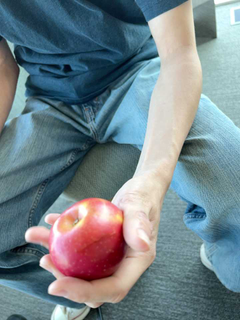
\includegraphics[width=1.30cm,height=1.80cm]{figures/chapters/ch01-basis/cofuse4d-method/assets/input_00118.png}};
    \draw[white,line width=.6pt] (0.95,3.05) rectangle ++(1.30,1.80);
    \draw[cfGray,line width=.35pt,dash pattern=on 1pt off 1pt] (0.55,3.95) -- (0.95,3.10);
    \draw[cfGray,line width=.35pt,dash pattern=on 1pt off 1pt] (0.55,3.95) -- (2.25,3.10);
    \foreach \x/\y/\r in {1.18/3.35/18,1.47/3.75/30,1.75/3.45/22,2.00/3.90/28}{%
      \draw[fill=cfOrange!22,draw=cfOrange,line width=.4pt,rotate around={\r:(\x,\y)}]
        (\x,\y) ellipse (.17 and .065);
    }
    \node[cfTiny,text=cfOrange] at (1.60,2.90) {渲染};
    \node[fill=cfOrange!18,draw=cfOrange,rounded corners=1.2pt,inner sep=1.6pt,
          font=\heiti\fontsize{6.6pt}{8pt}\selectfont,text=cfOrange] at (2.75,4.35) {RGB};
    \node[fill=cfBlue!12,draw=cfBlue,rounded corners=1.2pt,inner sep=1.6pt,
          font=\heiti\fontsize{6.6pt}{8pt}\selectfont,text=cfBlue] at (2.75,3.95) {Depth};
    \node[fill=cfGreen!14,draw=cfGreen,rounded corners=1.2pt,inner sep=1.6pt,
          font=\heiti\fontsize{6.6pt}{8pt}\selectfont,text=cfGreen] at (2.75,3.55) {Track};
    \node[cfTiny,anchor=west,text width=1.75cm] at (2.55,3.10) {光度 / 几何 / 轨迹监督};

    % 3) joint update and outputs
    \draw[fill=white,draw=cfGreen,line width=.7pt,rounded corners=2pt] (0.35,1.45) rectangle (1.75,2.05);
    \node[cfSmall,text=cfGreen] at (1.05,1.75) {GP 运动};
    \draw[fill=white,draw=cfOrange,line width=.7pt,rounded corners=2pt] (2.85,1.45) rectangle (4.25,2.05);
    \node[cfSmall,text=cfOrange] at (3.55,1.75) {高斯表示};
    \draw[cfGray,line width=.8pt,-{Latex[length=1.4mm,width=1mm]}] (1.82,1.88) .. controls (2.15,2.28) .. (2.78,1.88);
    \draw[cfGray,line width=.8pt,-{Latex[length=1.4mm,width=1mm]}] (2.78,1.62) .. controls (2.15,1.22) .. (1.82,1.62);
    \node[cfTiny,text=cfGray] at (2.30,2.18) {联合更新};
    \path[fill=cfOrange,rounded corners=2.2pt] (0.35,0.35) rectangle (4.35,1.18);
    \node[font=\heiti\fontsize{7.6pt}{9pt}\selectfont,text=white] at (2.35,0.90) {PCK@24 77.1 $\to$ 86.5};
    \node[font=\songti\fontsize{6.9pt}{8.2pt}\selectfont,text=white] at (2.35,0.57) {新视角合成 持平};
    \node[cfTiny,text=cfGray] at (2.35,0.18) {输出};
  \end{scope}

  % ================= arrows =================

\end{tikzpicture}
\endgroup

  \caption{CoFuse4D 的方法框架}
  \label{fig:cofuse4d-method}
\end{figure}

CoFuse4D 以连续时间高斯过程估计少量运动节点，并用轨迹级身份约束组织跨帧对应，再将对应关系共享于运动估计、高斯变形与渲染，通过重投影、光度和几何监督联合优化。在 DyCheck 七个场景上，24 像素阈值下轨迹命中率（PCK@24）由 77.15\% 提升至 86.54\%，新视角合成与冻结原始运动的参照重建基本持平。结果验证了连续运动与稠密对应融合的可行性，为本课题提供多时刻证据利用、置信度加权、连续查询及身份约束经验；对象边界、表面归属和观测不确定性仍待研究。该工作已基本完成，计划投稿至 CVPR 2027。

\noindent\textbf{（2）面向机器人操作的动作条件预测状态学习}

前期工作 PS-VLA 的论文题目为 \textit{PS-VLA: Learning Action-Conditioned Predictive States for Robotic Manipulation}。该工作在 BridgeVLA 的视觉-语言-动作框架\cite{ref12}上，研究机器人在连续执行中如何维护可预测、可修正的任务状态。BridgeVLA 主要依据当前多视角观测直接生成动作；当视觉观测存在较大不确定性或动作未产生预期效果时，仅依赖当前观测难以为后续决策保留一致的历史。PS-VLA 因此引入持续潜在状态：先根据上一时刻的后验、上一动作及实际执行反馈预测当前先验，再利用当前视觉 token 进行观测更新，得到后验状态。方法框架如图~\ref{fig:psvla-method} 所示。

\begin{figure}[H]
  \centering
  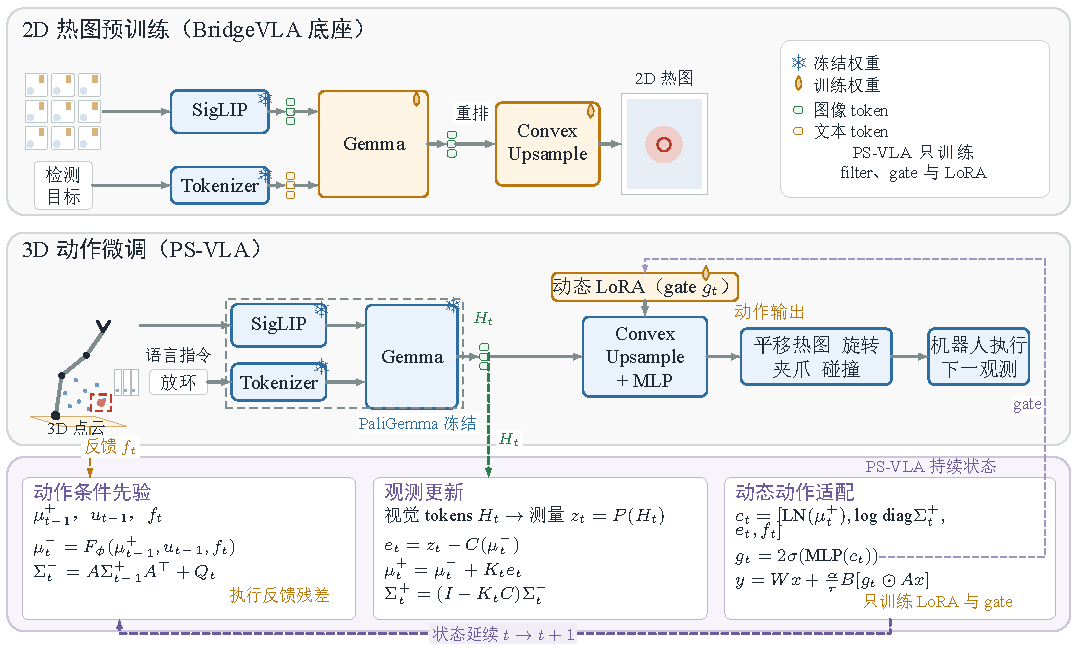
\includegraphics[width=\linewidth]{figures/chapters/ch01-basis/psvla-method/figure.pdf}
  \caption{PS-VLA 的方法框架}
  \label{fig:psvla-method}
\end{figure}

这一设计的核心是让状态在观测到来前先给出预测，再由新证据修正，而不是对当前帧重新编码或对历史无条件延续；实际执行反馈用于判断偏离来自观测噪声还是动作未按预期执行，使状态更新不必在“相信历史”和“相信当前观测”之间做固定选择。后验状态进一步通过动态 LoRA 的门控进入平移热图、旋转、夹爪和碰撞等动作头，使状态估计与动作适配共享同一更新链条。该工作为本课题第四项研究提供了状态转移、观测修正和动作条件适配的实现经验，也说明动作后果预测需要同时利用历史状态和当前证据。该工作已基本完成，计划投稿至 CVPR 2027。
